\section{Mission X}
	\subsection{Sous-mission X1}

	\begin{vwcol}[widths={0.8,0.2}, rule=0pt]
	\begin{minipage}{0.7\textwidth}
	\paragraph{Objectifs de la mission}

	Transformer l'image reçue par la sonde, pour savoir ce qui est arrivé à la sonde qui ne répond plus. Une image ressemblant à la transformée de Fourier de l'image originale a pu être récupérée.
	\end{minipage}
	\begin{minipage}{0.2\textwidth}
		\begin{flushright}
			\paragraph{Filtre utilisé}
		Transformée de Fourier inverse
		\end{flushright}
	\end{minipage}
	\end{vwcol} 

	\begin{figure}[h]
	\centering
		\begin{multicols}{2}
		
\includegraphics[scale=0.525]{images/X1.png}
		Avant
		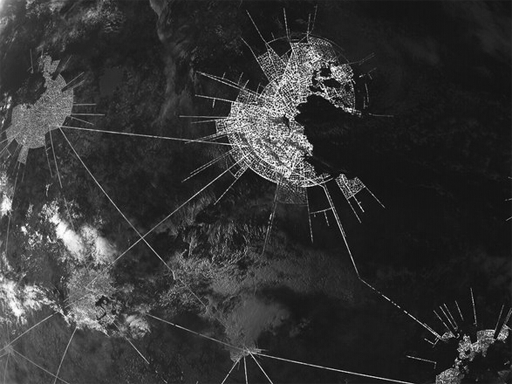
\includegraphics[scale=0.525]{images/X1AFTER.png}
		Après
		\end{multicols}
	\end{figure}
	\vspace{-0.9cm}

		\paragraph{Procédé}	
			Pour cette mission \emph{transformée de Fourier inverse} afin de retrouver l'image d'origine. La fonction native de Scilab \texttt{ifft} a été utilisée afin de faire l'opération inverse de transformation de Fourier. La fonction native a été utilisée pour sa rapidité et sa fiabilité.